\section{案例研究}
除了建立在基准测试集上的对照实验,我们也在更大规模的语料库 \ven~\cite{xu2017spreadcluster}上对 \wa 的检测有效性进行了案例研究。
\ven 包含 1,609 个由多个电子表格构成的演化组(组里的每个电子表格都是最初的一个电子表格在维护过程中的特定版本),是从 Enron 电子表格数据库\cite{hermans2015enron}里的 79,983 个工作表中提炼而来。
我们从每个演化组中选取最新的电子表格文件,总共包含 1,609 个电子表格,其中含 7,140 个工作表,作为我们案例研究的测试对象。
我们把不同的电子表格缺陷检测技术拿来检测这些工作表,进而比较和分析它们的检测效果。
考虑到 \uc 和 \di 检测出的缺陷数量极少(低于总量的 1\%),在案例研究中我们选择了剩余四种技术来进行实验,即\am 、\ca、\cu 和 \wa。
为了保证对比的公平性,我们移除了那些至少有一个技术无法正常执行的工作表(比如:测试该工作表时,导致程序异常崩溃,或者超出了我们设定的每张工作表五分钟执行时间上限,设置时限的目的是防止程序陷入死锁或者其他未知的错误而影响整体实验进度)。
这一过滤数据集的方式给我们的案例研究最终留下了总计 6,258 个工作表。

我们注意到 \ven 并不包含用于评估电子表格缺陷检测技术有效性的人工标注结果(即,每张工作表里实际含有哪些有缺陷的单元格是未知的)。
因此,我们主要关注 4 个技术的缺陷检测精度。
另外,由于整体数据量庞大,虽然我们对每个工作表都运行了检测程序(用于衡量他们的时间效率),但我们不得不使用采样的方法来选择少量工作表,进行人工参与的检测精度统计。
采样过程遵循了 \am 和 \cu 建议的数据收集方式。
在所有 6,258 个工作表中, 1,525 个工作表被至少一个技术检测出含有缺陷。
基于此,我们随机采样了约 20\% 的工作表(即 300 个工作表)来进行人工审查,该审查的目的是标注每一个被工具报告出来有缺陷的单元格是真阳性或假阳性。

\subsection{检测耗时和采样分析}
表\ref{table5}对比了 4 个技术在人工审查后的缺陷检测结果。

从表\ref{table5}的左半部分,我们可以观察到:
\wa 检测出了最少数量的缺陷单元格(9,462个),对比于 \am 的 20,280个、\ca 的 12,953个 和 \cu 的 14,102个。
考虑到 \wa 在前面的基准测试集中获得了最高的检测精度,在此次案例研究中,\wa 也符合高精度的预期:在 \wa 检测出的 1,240 个缺陷单元格中有 512 个真阳性,相比较而言,在 \am 检测出的 3,316(是 \wa 的 2.6 倍) 个缺陷中仅有 540 个真阳性(仅是 \wa 的 1.05 倍)。
考虑到时间效率,\am 处理所有的 6,258 个工作表所花费时间最短(仅 21 分钟),其他三个技术都花了相对长的时间(从 351 到 516分钟)。
这结果表明 \am 适合用于快速识别潜在的电子表格缺陷,但因为他的检测质量相对较低(精度是 16.3\%),它更适合作为其它技术的补充验证来使用(比如用于过滤大多数的假阳性缺陷)。
\wa 的执行时间也没有那么高效(花费 518 分钟),对比于 \cu 的时间消耗(537分钟)。
消耗时间减少的原因是:\wa 移除了不相关的单元格和不合格的单元格类,节省了后续的缺陷检测时间,这一努力带来了运行时间的略微缩短(19分钟)。

\begin{table}[tbp]
    \centering
    \caption{在 VEnron2 数据集上四个电子表格缺陷检测技术的检测结果}
    \label{table5}
    %\large
    \resizebox{\columnwidth}{!}{
    \begin{tabular}{|m{.15\columnwidth}<{\centering}|m{.16\columnwidth}<{\centering}|m{.16\columnwidth}<{\centering}|m{.14\columnwidth}<{\centering}|m{.12\columnwidth}<{\centering}|m{.1\columnwidth}<{\centering}|m{.12\columnwidth}<{\centering}|}
    \hline
    ~& \multicolumn{3}{c|}{\textbf{全部数据集包含 6,258 个工作表}} & \multicolumn{3}{c|}{\textbf{采样 300 个工作表}} \\
    \hline
    \textbf{技术} & \textbf{\# 工作表} & \textbf{\# 缺陷} & \textbf{耗时 (分钟)} & \textbf{\# 缺陷} & \textbf{\# TP} & \textbf{Precision} \\
    \hline
        AmCheck  & 859  & 20,280 & 21 & 3,316 & 540 & 16.3\% \\
    \hline
        CACheck  & 953   & 12,953 & 372 & 1,559 & 534 & 34.3\% \\
    \hline
        CUSTODES & 1,284 & 14,102 & 537  & 2,334 & 629 & 26.9\% \\
    \hline
        WARDER   & 1,136 & 9,462  & 518  & 1,240 & 512 & 41.3\% \\
    \hline
    \end{tabular}}
\end{table}
\begin{figure}[tp]
    \centering
    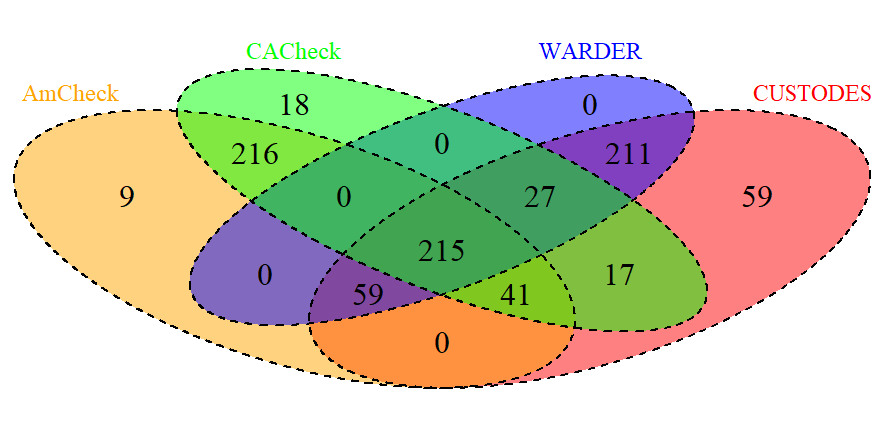
\includegraphics[width = 0.9\columnwidth]{figure/figure10.png}
    \caption{四个电子表格缺陷检测技术报告出的真阳性交集的韦恩图}
    \label{figure10}
\end{figure}

从表\ref{table5}的右半部分,我们可以观察到:
\begin{enumerate}
    \item 在 4 个技术中,\wa 取得了最高的缺陷检测精度(41.3\%),超出其他技术7.0-25.0\%,这和之前我们验证过的 \wa 更加关注于在 \cu 的基础上提升精度的结论(41.3\% vs. 26.9\%);
    \item 尽管 \wa 报告了更少的真阳性数量(512个),但同时也伴随着少得多的假阳性数量(728个),这比其他技术的假阳性数量少了 297-2,048 个,这一特性在现实场景可能相当实用,因为所有的电子表格缺陷必须经过人工的审核验证,节省了大量人力消耗。
\end{enumerate}

因此,\textit{\wa 在实际使用的电子表格上的缺陷检测表现也相对令人满意。它获得了最高的检测精度(41.3\%),超出其它技术达 7.0-25.0\%。尽管它的时间消耗有点高,但也和 \ca 相当(在同一个量级),并且少于它的前身 \cu。}

\subsection{技术的互补性}
如图\ref{figure10}中的韦恩图所示,除了整体的检测精度和时间消耗对比,我们也研究了四个技术检测出的真阳性交集。
在韦恩图中,黄色椭圆代表 \am 检测出的真阳性缺陷,依次地,绿色椭圆代表\ca 、粉色椭圆代表\cu 、紫色代表 \wa 。
每个子区域代表两个或多个技术检测出的真阳性缺陷的交集。
从图中,我们可以观察出:
\begin{enumerate}
    \item 基于模板匹配的技术(\am 和 \ca)和基于聚类学习的技术(\cu 和 \wa)明显彼此互补。
    前者总共检测出 243(9+216+18)个无法被后者检测出的缺陷,而后者检测出 270(211+59)个前者无法检测的缺陷。
    此结果表明两类技术都很有用处;

    \item 在基于模板的技术中,\ca 继承自 \am 技术。相应地,它们检测出的缺陷有一大部分是相同的(78.4\%,602 个中的 472 个是相同的)。
    因此,\am 单独检测出 68 个缺陷,而 \ca 单独检测出 62 个。
    不过,\ca 仍是更受欢迎的技术,考虑到它显著减少了假阳性(从\am 的 2776 个减少到 1025 个);
    
    \item 在基于学习的技术中,\wa 检验了 \cu 的检测结果。相应地,\wa 仅检测出了 512 个真阳性,是 \cu 的子集(81.4\%)。
    不过,\wa 本身就是更加关注与过滤掉不相关的单元格和不合格的类,并且这一努力带来了显著的假阳性的减少(从 \cu 的 1,705 个减少到 728 个);
    
    \item \ca 和 \wa 作为各技术流派的代表,仍然是可以相互补充的。
    它们各自能够检测出 292 个和 270 个对方无法检测出的缺陷。
    这一结果很明确地表明它们的互补性很强。
\end{enumerate}

因此,\textit{就检测到的缺陷而言,所有相关技术都有它们各自的优势,并且精细的案例研究结果表明他们是可以彼此互补使用的。}
